\documentclass[a4paper,10pt]{article}
\usepackage[margin=3cm]{geometry}
\usepackage{amsmath}
\usepackage{fancyhdr}
\usepackage{hyperref}
\usepackage{graphicx}
\usepackage{float}

%opening
\pagestyle{fancy}{
\fancyhf{}
\fancyhead[L]{\textit{}}
\fancyhead[R]{\textsc{\nouppercase{\leftmark}}}
\cfoot{\thepage}
}
\title{}
\author{}
\setcounter{tocdepth}{2}

\begin{document}

\maketitle
Comparison DoA.
%\thispagestyle{empty}
\begin{abstract}
	
\end{abstract}
%\tableofcontents
The comparison of the beamforming operated using real angles and DoA shows some differences in the situations that we analyze.

We start taking in exam “UPDATEphsDoALMSCompareWithKnownMovement.m”: here it is possible to see that the differences are very minimal: in fact here it is possible to see that the differences depend only on the precision of the scan step angle made by the MUSIC estimator: it means that, since our scanning angle is 0.5°, if the angle measure a value in the slot of scanning, it will be rounded to the considered value, giving rounding error: for example, having a value that will be 0.4°, it will be rounded to 0.5°; this delta affects the precision of the beamforming, and could be very small, generating beams that cover almost everytime the target that we use in our scenario.
 
 We can see it in the image of the beam, where continuous lines are the ones representing the DoA beamforming, and the dotted ones represent the beamforming made with real angles, noting that the two lines are near, sometimes indistinguishable:
\begin{figure}[H]
	\centering
	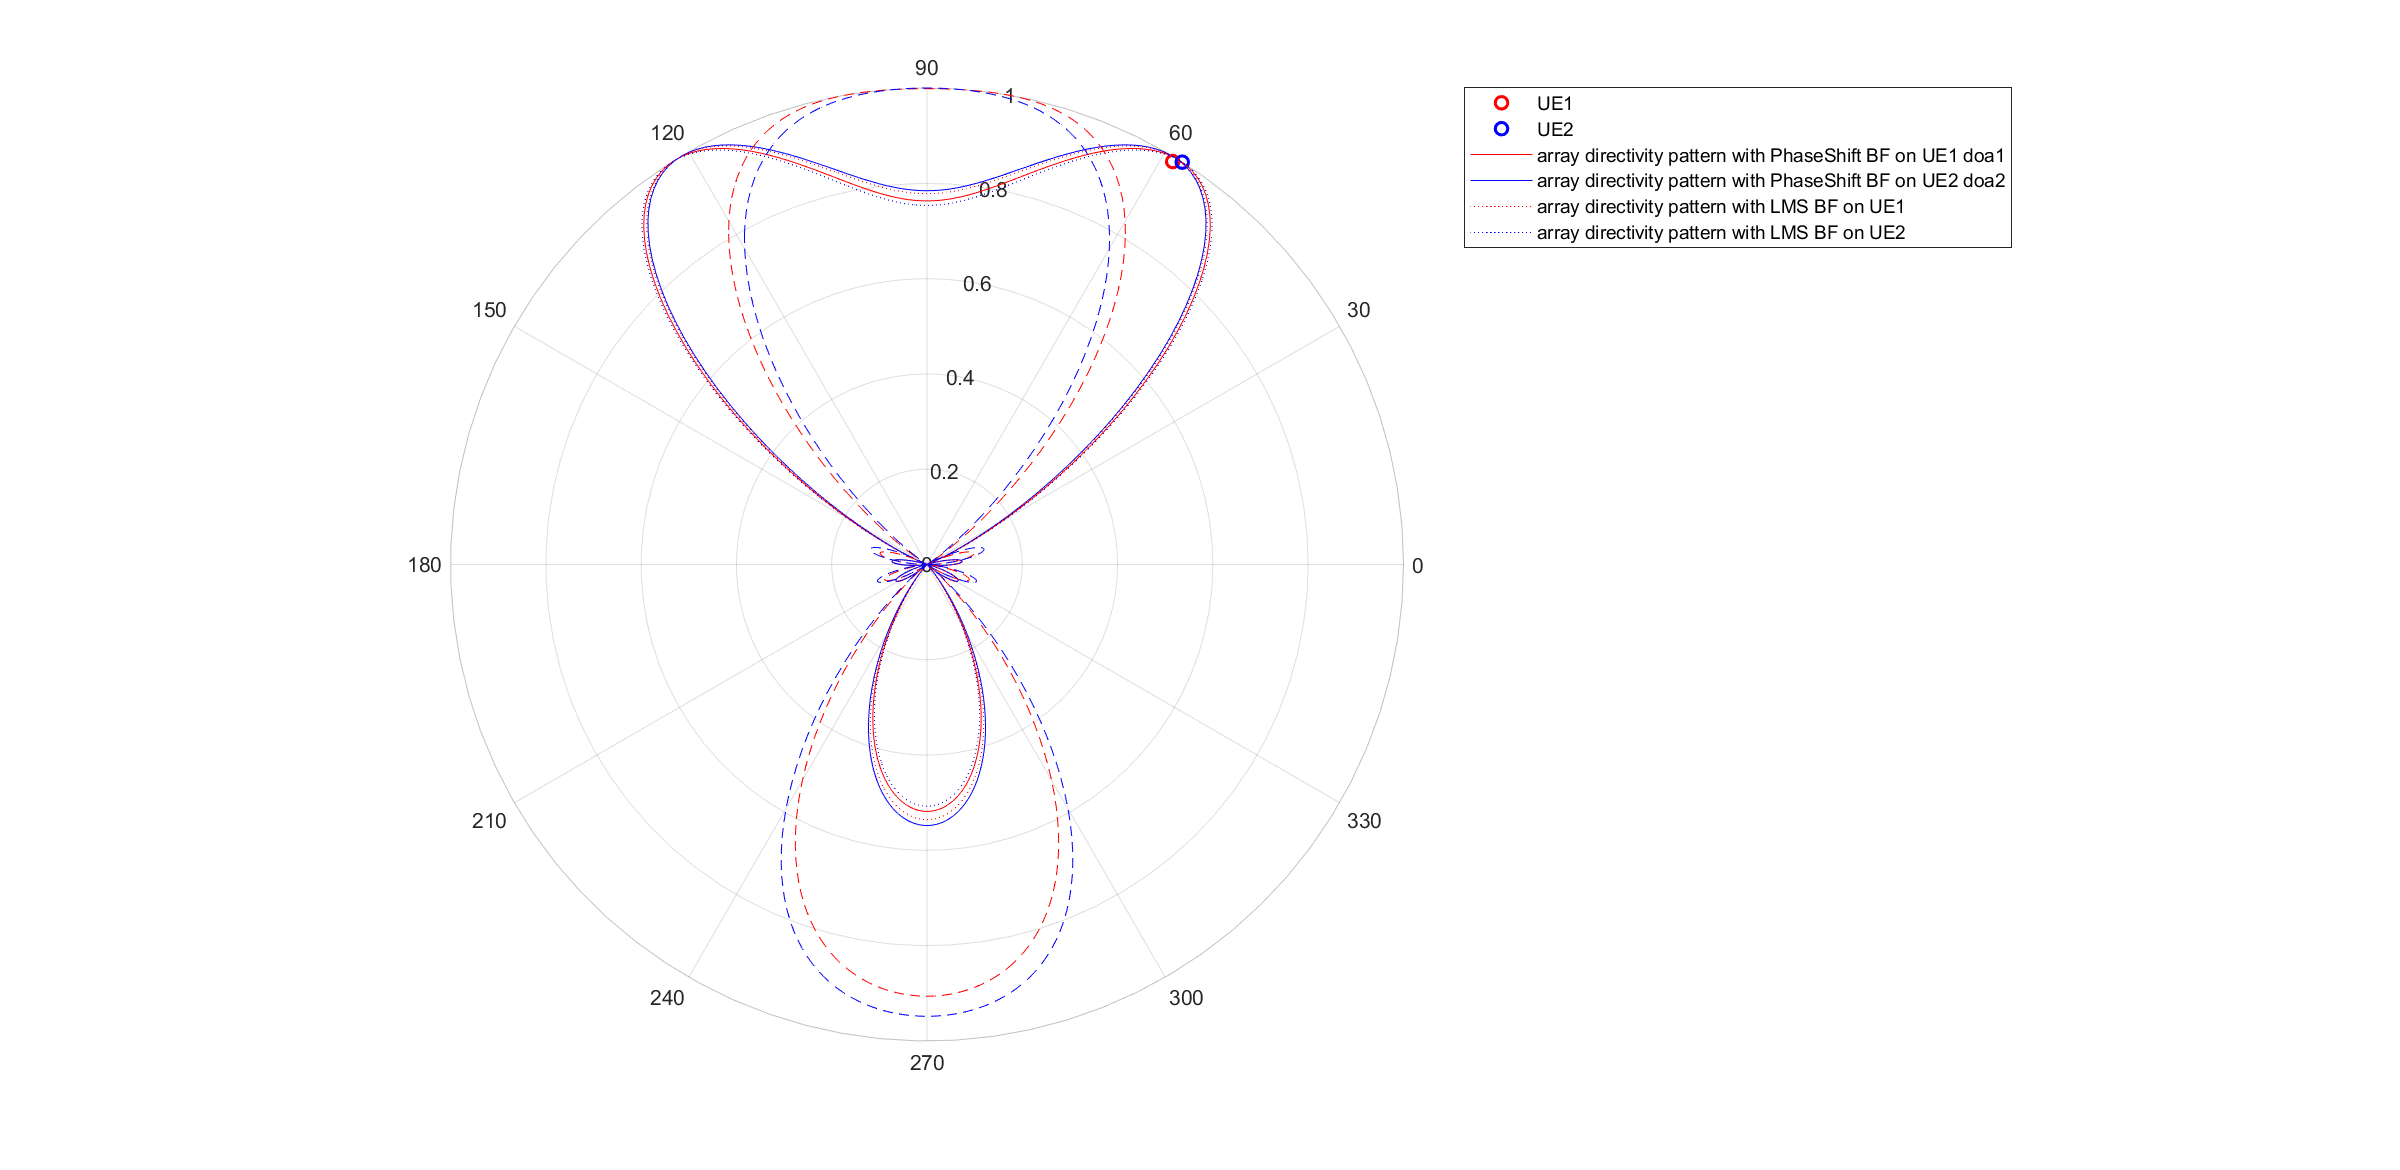
\includegraphics[width=0.8\linewidth]{polarplot60.png}
	\caption{\label{fig:polarplot60}the precision of beamforming of DoA without interferences, compared to the case of real angles.}
\end{figure}

Now we can take in exam “UPDATEphsDoALMSWithKnowNumberOfInterferences.m”: here the situation changes deeply: in fact, what happens is that the presence of the interferences affects the estimation with an error greater than the case where there aren't: the geometry of the system is essential to understand what happens: having a great distance between the interferences and the targets, gives the possibility to make a beanforming that is less accurate than the previous case, but quite accurate to distinguish the angles, with an inaccuracy of at most some grades, given by the presence of the interferences in the signal that arrives in the BS.

\begin{figure}[H]
	\centering
	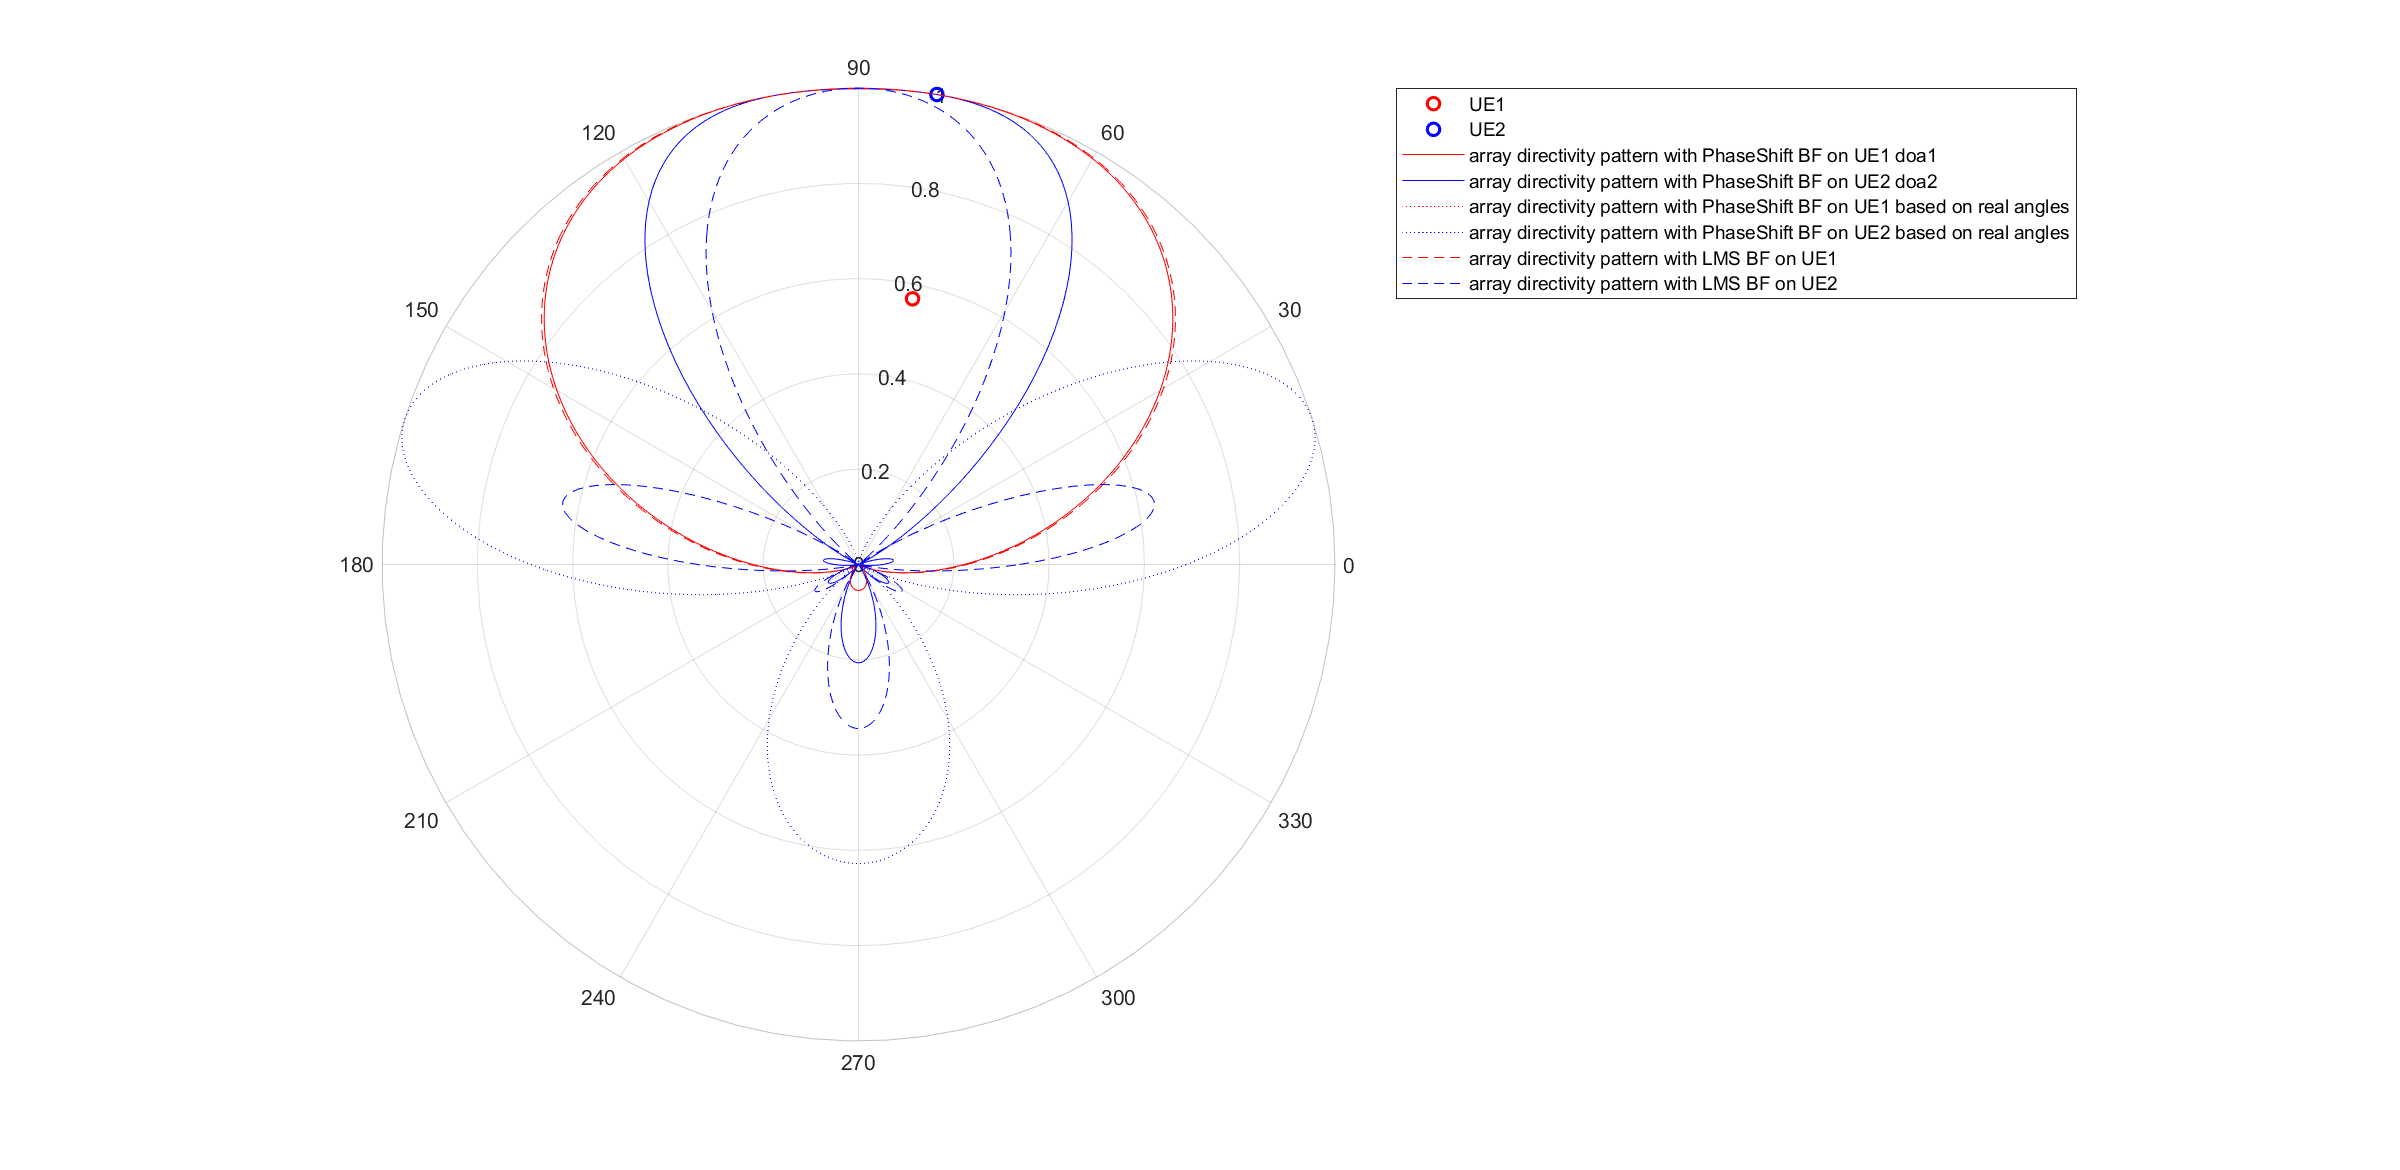
\includegraphics[width=0.8\linewidth]{complete_polarplot8.png}
	\caption{\label{fig:complete_polarplot8} an accurate estimation of the position of the targets, in a scenario with interferences.}
\end{figure}

In case of proximity of the interferences to the targets, it happens that the MUSIC estimator is not able to distinguish the interferences to the targets, so it presents some angles that could be very different than the real ones, influenced by the position of the less interferred target, that dominate the estimation: so instead of have two different pair of azimuth-elevation angles, it could be possible to have the angles referring to one target with little difference of degrees, that could be in the order of some fraction of degree, to some degrees.

This consideration could be see in the graph of Beamforming by the fact that beams, in contrast to the case of no interferences, are quite different than the real angles case, and in case of proximity could make the estimation of only one target, the dominant one.

\begin{figure}[H]
	\centering
	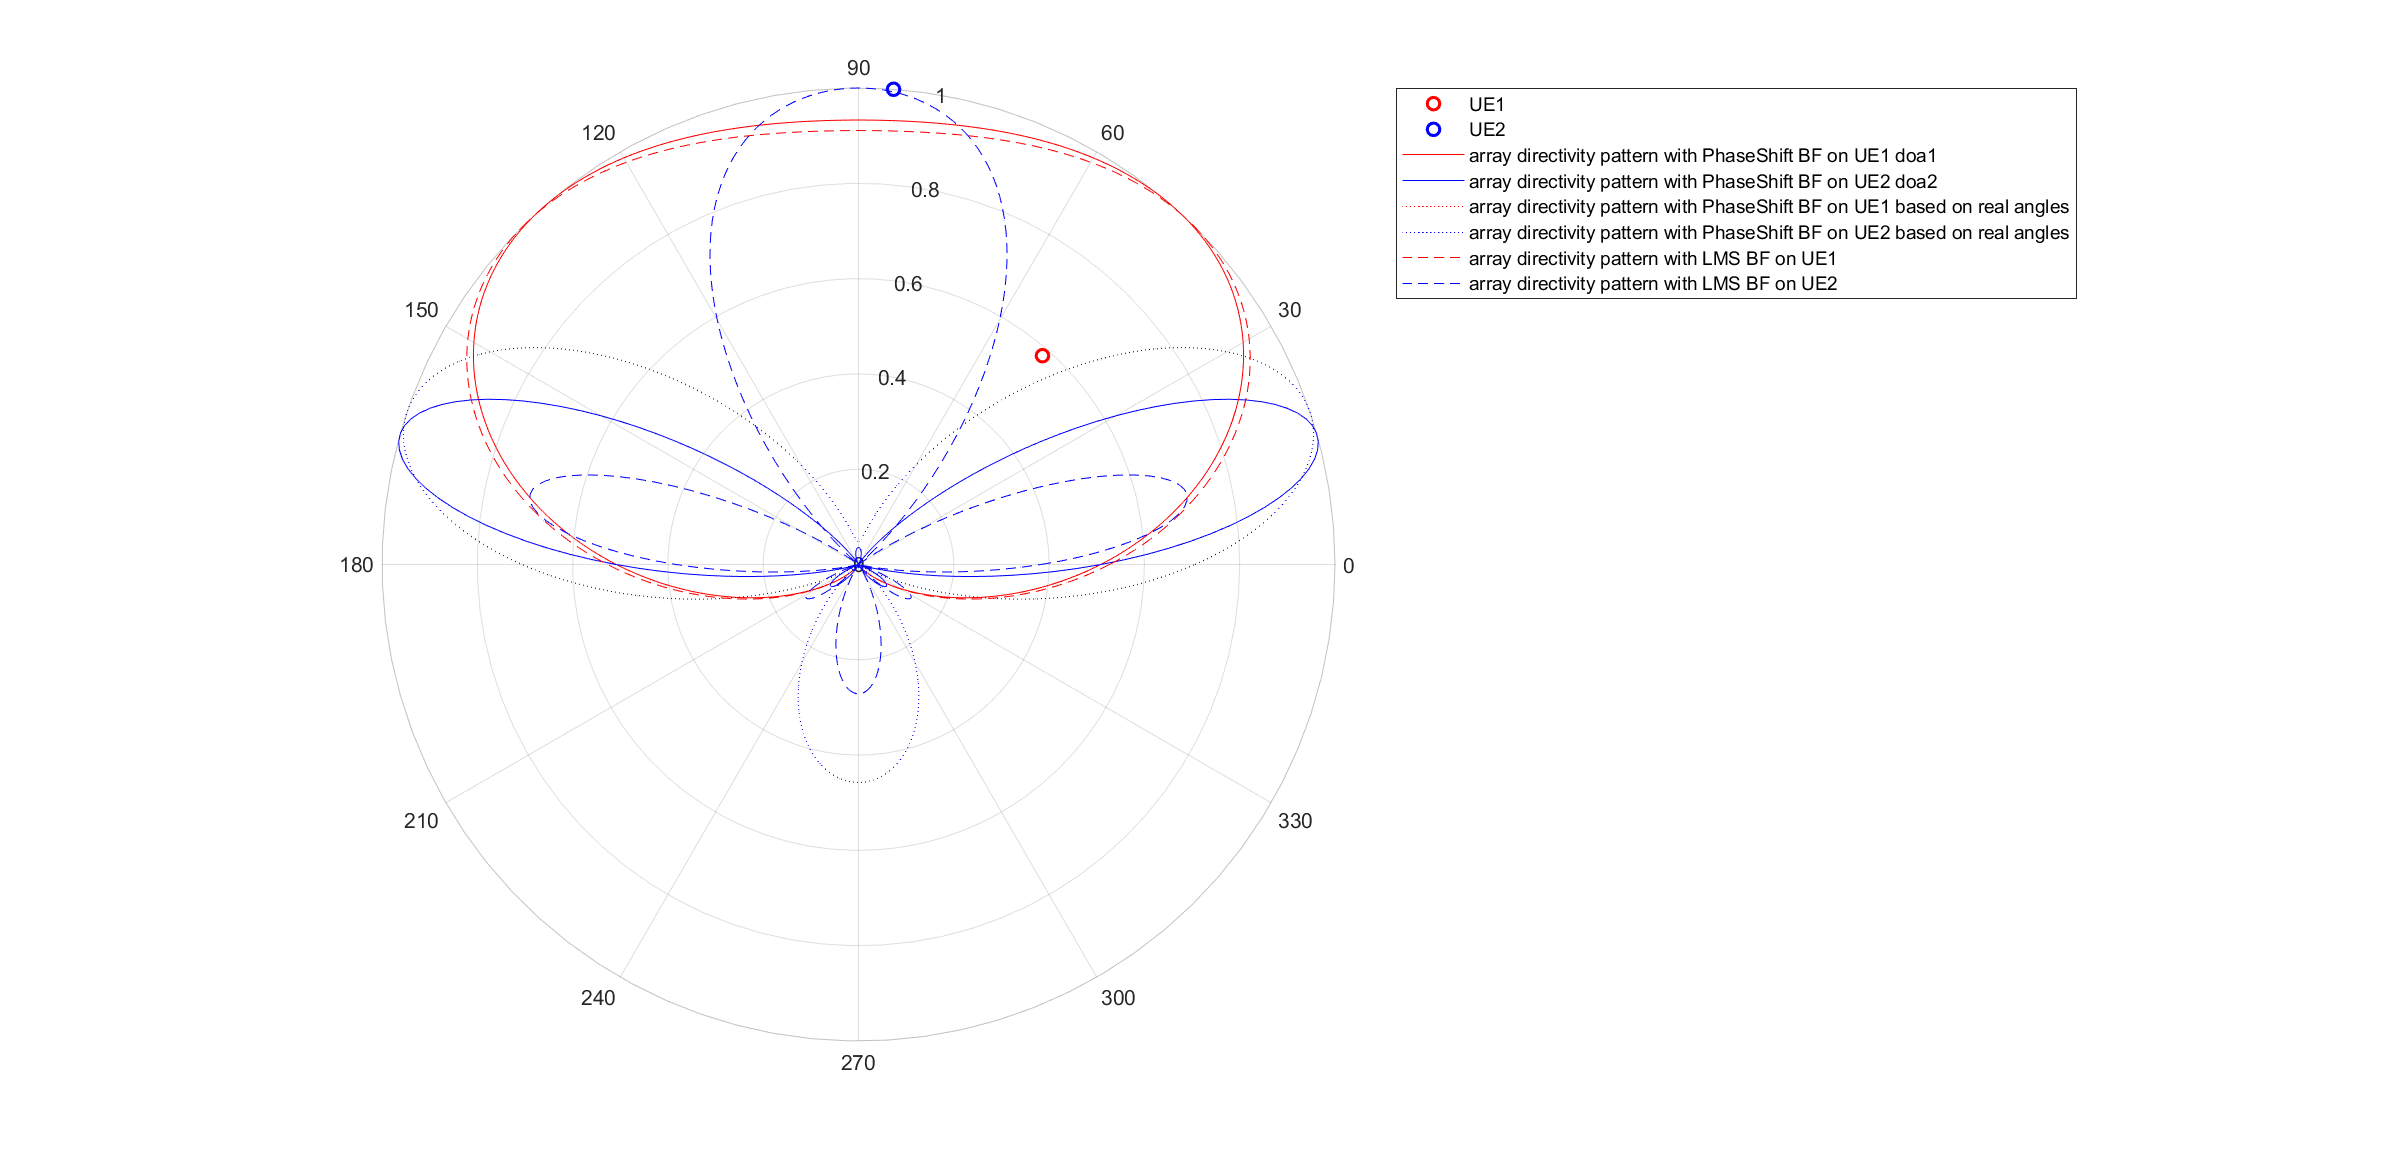
\includegraphics[width=0.8\linewidth]{complete_polarplot6.png}
	\caption{\label{fig:complete_polarplot6}the inaccuracies of the estimation of DoA for the position of UE2}
\end{figure}
\end{document}
